\subsection{(W) Mission Control Run}\label{s:missionControlRun}
    \noindent Cover algorithm outer run in multiple decision frames (As bonus mark decision points for rule engine \emph{decision points}):
    \begin{itemize}
        \item Waypoint reach condition
        \item Waypoint waver condition (when to give up on chasing unreachable dream)
        \item Trajectory selection criteria in inner avoidance run
        \item Complete mission control run, including decision invocation conditions
        \item Basically MissionControl.runMissionOnce() function in detail
		\item The navigation concept taken from \cite{sabatini2014navigation,Sabatini2014}.
    \end{itemize}
    \noindent Decision invocation conditions:
    \begin{itemize}
        \item Empty movement Buffer (go to Emergency mode)
        \item New static obstacle/constraint detection (go to Emergency mode)
        \item Active moving obstacle (Depending on mode)
        \item In Cooperative Navigation mode - Avoidance grid not empty
        \item In Emergency avoidance mode - Avoidance grid is empty
    \end{itemize}
    \begin{figure}[H]
	    \centering
        \begin{subfigure}{0.48\textwidth}
            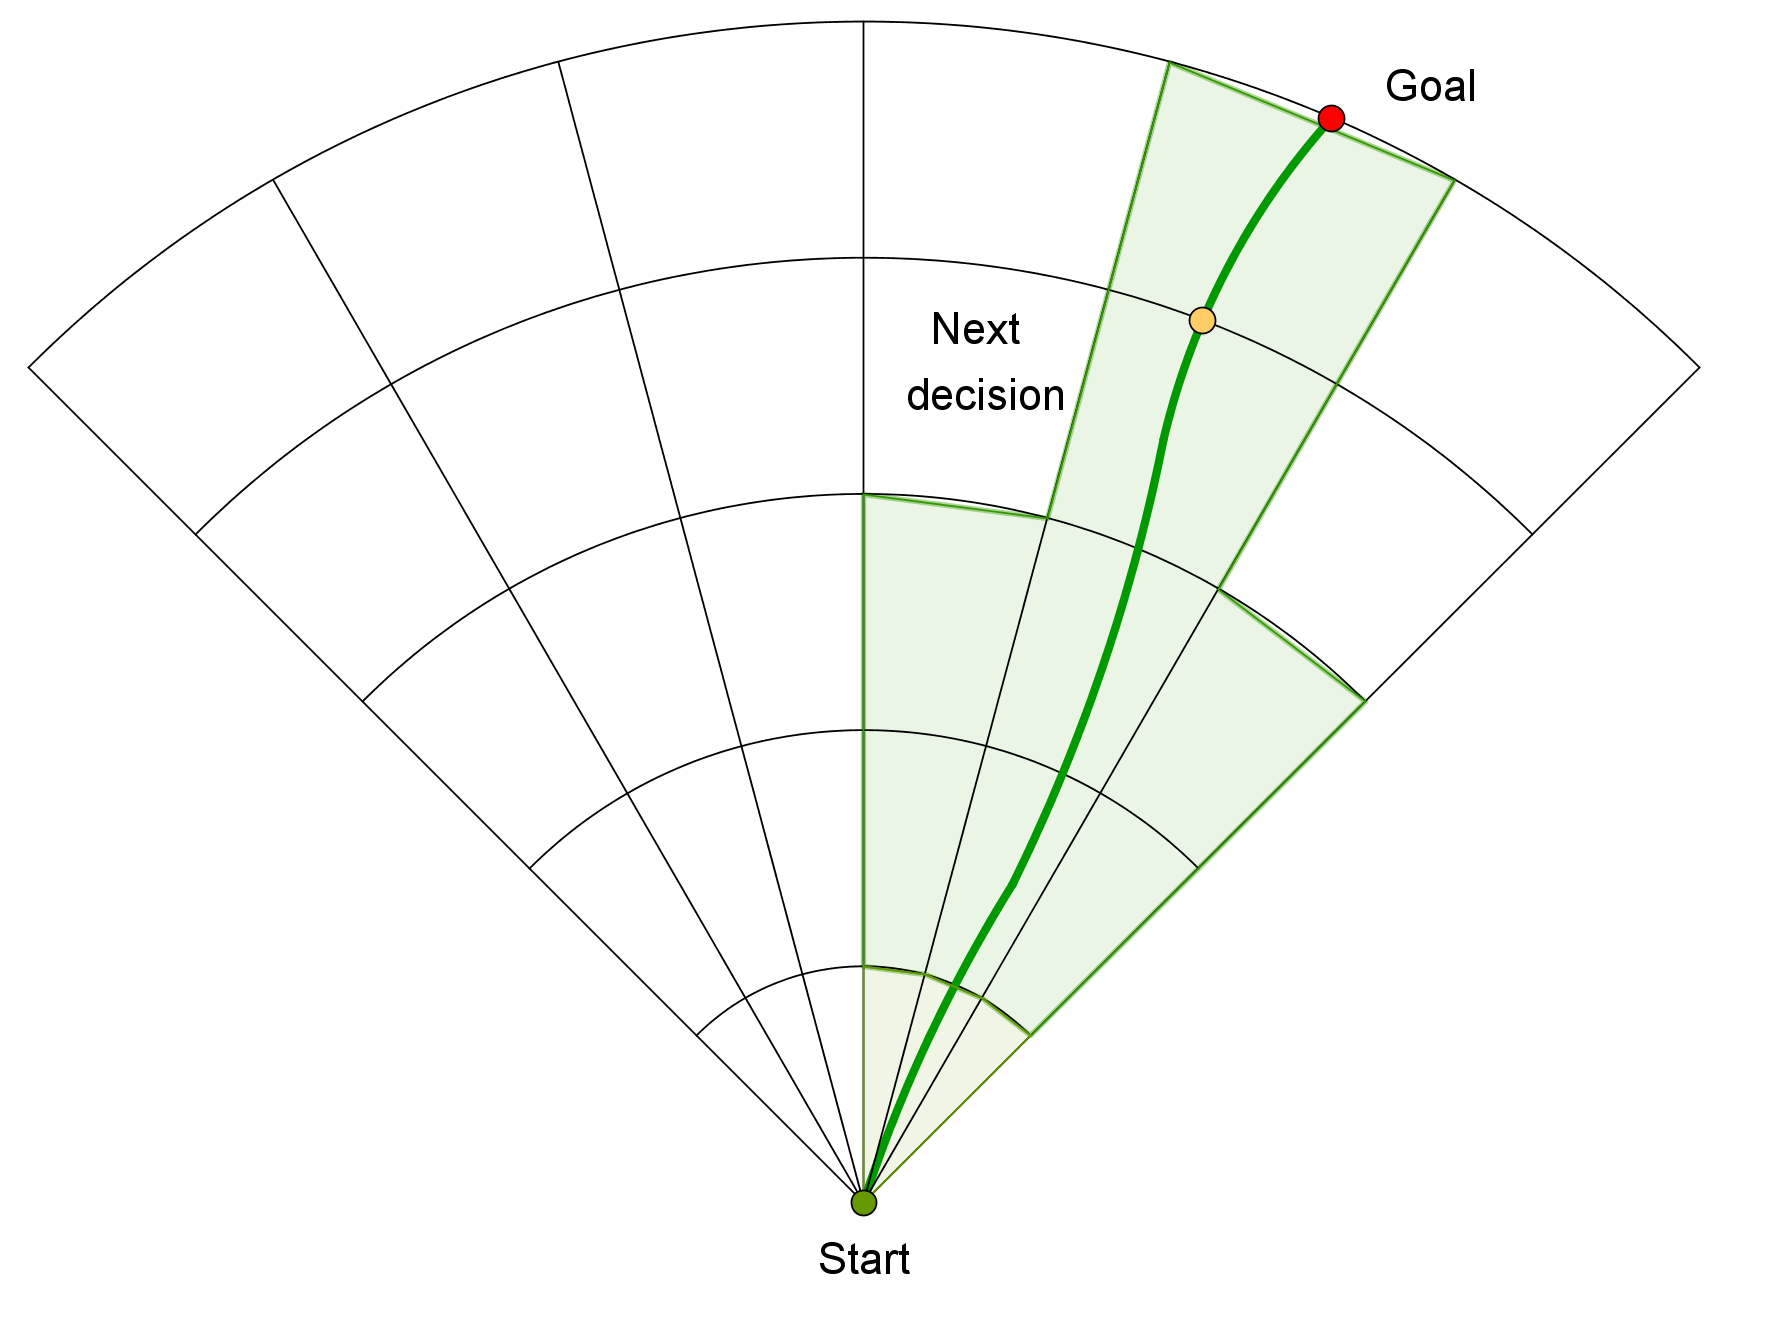
\includegraphics[width=0.9\linewidth]{\FIGDIR/CA005PathCalculation}
            \caption{Mission control run example.}
            \label{fig:missionControlRunExample}
        \end{subfigure}
        \begin{subfigure}{0.48\textwidth}
            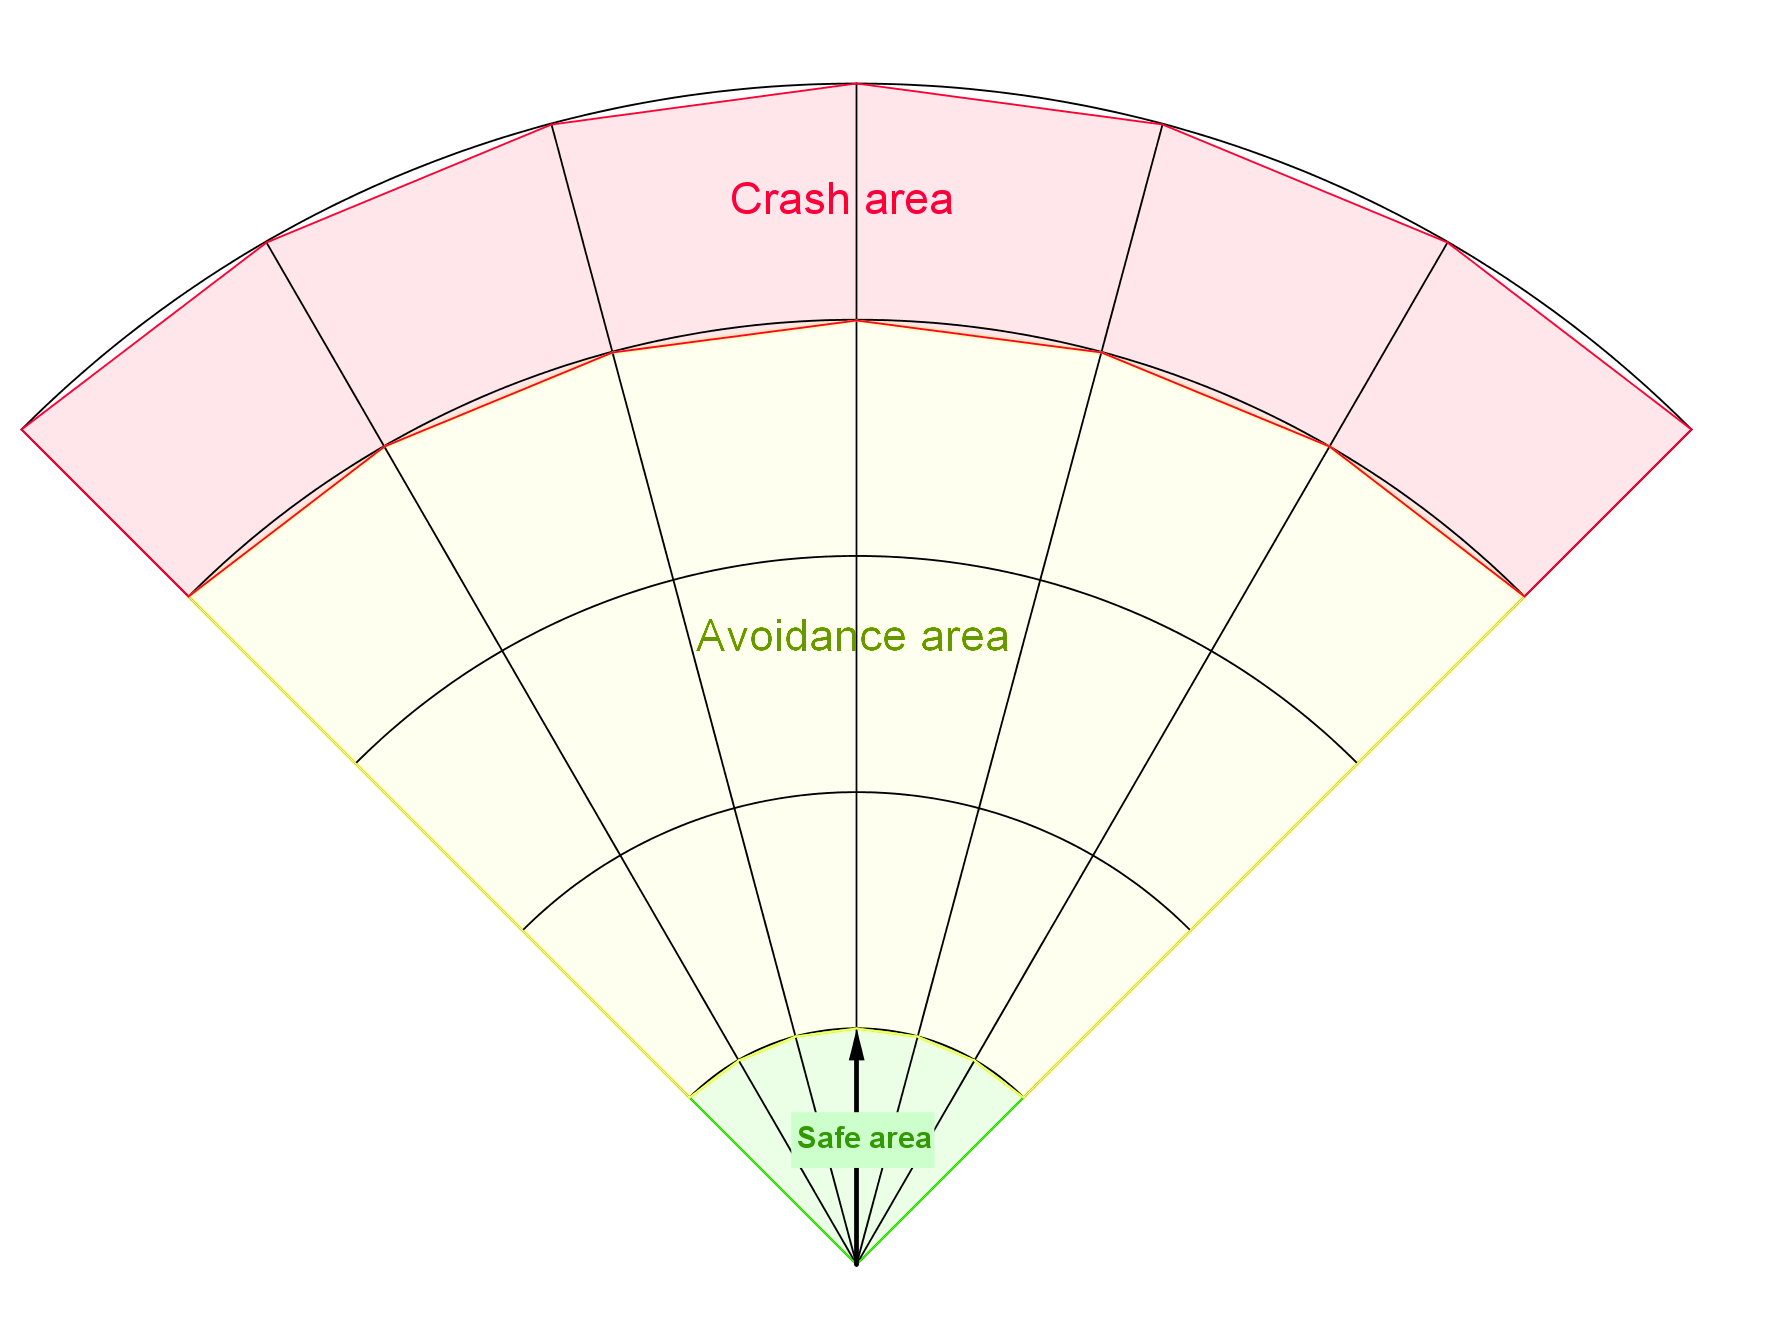
\includegraphics[width=0.9\linewidth]{\FIGDIR/CA006FieldOfViewZones} 
            \caption{Grid zones.}
            \label{fig:gridZonesMissionControl}
        \end{subfigure}
        \caption{Definitions for \emph{Mission Control Run} (outer loop).}
        \label{fig:definitionsForMissionControlRun}
    \end{figure}
    
    \begin{figure}[H]
        \centering
        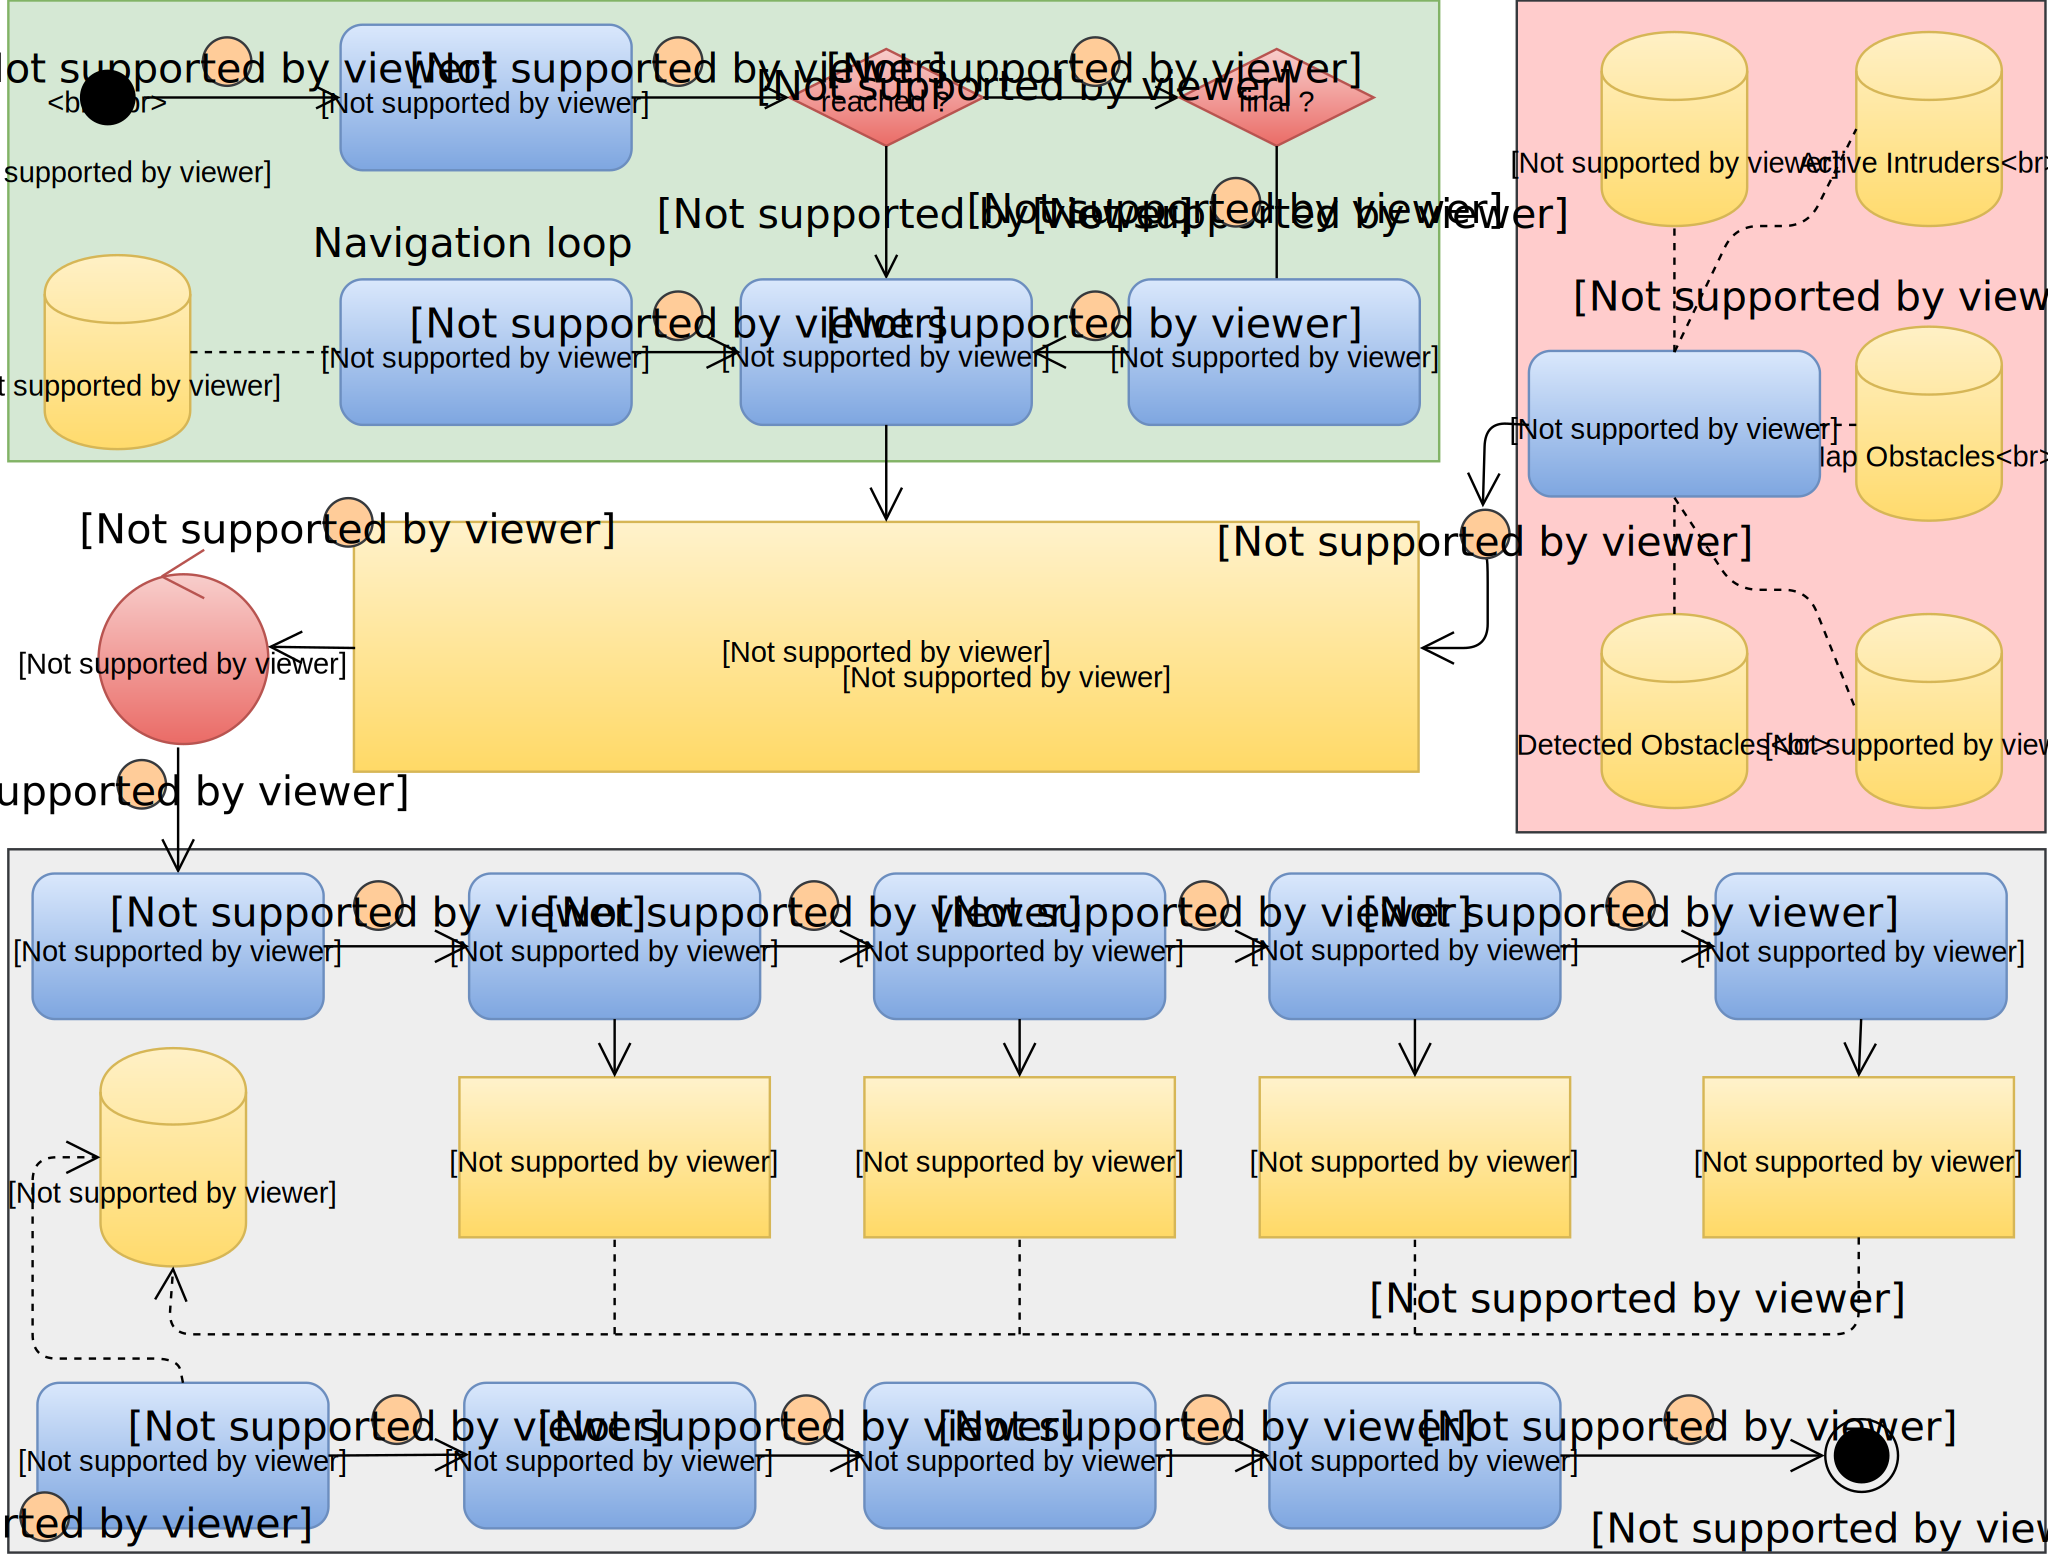
\includegraphics[width=\linewidth]{\FIGDIR/TE026AvoidanceAlgorithmMainLoopRun}
        \caption{Mission control run activity diagram.}
        \label{fig:missionControlRunActivityDiagram}
    \end{figure}

